\documentclass[11pt]{article}

% -*- TeX-master: "Informe.tex" -*-


\usepackage[margin = 1in]{geometry}
\usepackage[utf8]{inputenc}
\usepackage[T1]{fontenc}
\usepackage[spanish, es-tabla]{babel}
\usepackage[spanish]{varioref}
\usepackage{fancyhdr}
\usepackage[colorlinks, linkcolor = blue]{hyperref}
\usepackage{graphicx}
\usepackage{wrapfig, caption, subcaption}
\usepackage{booktabs}
\usepackage[dvipsnames, table]{xcolor}
\usepackage{minted}
\usepackage{tikz}
\usepackage{dirtree, fontawesome}
\usepackage{soul}
\usepackage{outlines}


\usetikzlibrary {
  trees,
  matrix,
  positioning,
  external,
  fit,
  backgrounds,
  arrows,
}
\tikzexternalize[prefix = Figures/]

\tikzset{
  tree/.style = {
    level distance = 5cm,
    sibling distance = 7cm,
    ->,
    ultra thick,
    ampersand replacement = \&
  },
  board/.style = {
    matrix of nodes,
    row sep = -\pgflinewidth,
    column sep = -\pgflinewidth,
    -,
    nodes = {rectangle, draw = black, fill = blue!15, align = center},
    ultra thick,
    font = \Huge\bf,
    minimum size = 1.1cm,
    % nodes in empty cells,
    ampersand replacement = \&
  },
  marker/.style = {
    opacity = .4,
    -,
    line width = 7mm,
    line cap = round,
    color = #1
  },
  cross/.style = {
    -,
    line width = 4mm,
    color = red
  },
  fig/.style = {
    circle,
    draw = black!70,
    very thick
  },
  line/.style = {
    ->,
    very thick
  },
  unir/.style = {
    <->,
    ultra thick,
  },
}

\tikzset{
  box/.style = {
    rectangle,
    draw = #1!75,
    fill = #1!30,
    inner sep = 5pt,
    very thick
  },
  boxp/.style = {
    rectangle,
    draw = #1,
    fill = #1!60,
    inner sep = 5pt,
    very thick
  },
  cont/.style = {
    shape = rectangle,
    align = center,
    draw  = #1,
    fill  = #1!10,
    rounded corners,
    inner sep = 8pt
  },
  con/.style = {
    -stealth,
    very thick
  }
}

\newcommand{\connectV}[2]{
  \draw[con] ([xshift = -10pt]#1.south) to ([xshift = -10pt]#2.north);
  \draw[con] ([xshift = 10pt]#2.north) to ([xshift = 10pt]#1.south);
}

\newcommand{\connectH}[2]{
  \draw[con] ([yshift = -8pt]#1.east) to ([yshift = -8pt]#2.west);
  \draw[con] ([yshift = 8pt]#2.west) to ([yshift = 8pt]#1.east);
}

\newmintedfile[pycode]{python} {
  frame = single,
  framerule = 1.25pt,
  framesep = 3mm,
  bgcolor = black!6,
  fontsize = \small,
  linenos = true,
  % numberblanklines = false,
  numbersep = 1pt,
  xleftmargin = \parindent,
  breaklines,
  tabsize = 4,
  obeytabs = false,
  mathescape = true,
  samepage = false,
  showspaces = false,
  showtabs = false,
  texcl = false,
  labelposition = all,
}

\newmintedfile[phpcode]{html+php} {
  frame = single,
  framerule = 1.25pt,
  framesep = 3mm,
  bgcolor = black!6,
  fontsize = \small,
  linenos = true,
  % numberblanklines = false,
  numbersep = 1pt,
  xleftmargin = \parindent,
  breaklines,
  tabsize = 4,
  obeytabs = false,
  mathescape = true,
  samepage = false,
  showspaces = false,
  showtabs = false,
  texcl = false,
  labelposition = all,
}

\newmintedfile[htmlcode]{html} {
  frame = single,
  framerule = 1.25pt,
  framesep = 3mm,
  bgcolor = black!6,
  fontsize = \small,
  linenos = true,
  % numberblanklines = false,
  numbersep = 1pt,
  xleftmargin = \parindent,
  breaklines,
  tabsize = 4,
  obeytabs = false,
  mathescape = true,
  samepage = false,
  showspaces = false,
  showtabs = false,
  texcl = false,
  labelposition = all,
}

\newmintedfile[csscode]{css} {
  frame = single,
  framerule = 1.25pt,
  framesep = 3mm,
  bgcolor = black!6,
  style = colorful,
  fontsize = \small,
  linenos = true,
  % numberblanklines = false,
  numbersep = 1pt,
  xleftmargin = \parindent,
  breaklines,
  tabsize = 4,
  obeytabs = false,
  mathescape = true,
  samepage = false,
  showspaces = false,
  showtabs = false,
  texcl = false,
  labelposition = all,
}

\newmintedfile[jscode]{js} {
  frame = single,
  framerule = 1.25pt,
  framesep = 3mm,
  bgcolor = black!6,
  style = colorful,
  fontsize = \small,
  linenos = true,
  % numberblanklines = false,
  numbersep = 1pt,
  xleftmargin = \parindent,
  breaklines,
  tabsize = 4,
  obeytabs = false,
  mathescape = true,
  samepage = false,
  showspaces = false,
  showtabs = false,
  texcl = false,
  labelposition = all,
}

\renewcommand{\theFancyVerbLine}{\sffamily \small \arabic{FancyVerbLine}}


\newcommand{\imgInline}[1]{\includegraphics[height = 1.25\fontcharht\font`\B]{#1}}

\newcommand{\myFolder}[1]{\faFolderOpen\ {#1}}
\newcommand{\myFile}[1]{\faFileTextO\ {#1} }
\newcommand{\myPdf}[1]{\faFilePdfO\ {#1.pdf}}
\newcommand{\myZip}[1]{\faFileZipO\ {#1.zip}}
\newcommand{\myPy}[1]{\faFileTextO\ {#1.py} \imgInline{Logo_Python.png}}
\newcommand{\myJs}[1]{\faFileTextO\ {#1.js} \imgInline{Logo_JS.png}}
\newcommand{\myPhp}[1]{\faFileTextO\ {#1.php} \imgInline{Logo_PHP.png}}
\newcommand{\myHtml}[1]{\faFileTextO\ {#1.html} \imgInline{Logo_HTML.png}}
\newcommand{\myCss}[1]{\faFileTextO\ {#1.css} \imgInline{Logo_CSS.png}}
\newcommand{\myImg}[1]{\faFileImageO\ {#1.png}}


\newlength\tindent
\setlength{\tindent}{\parindent}
\setlength{\parindent}{0pt}
\renewcommand{\indent}{\hspace*{\tindent}}

\pagestyle{fancy}
\renewcommand{\footrulewidth}{0.4pt}
\lhead{\slshape Tres en Raya con Raspberry Pi}
\rhead{\slshape\nouppercase{\leftmark}}
\cfoot{David Álvarez, Guillermo Creus}
\rfoot{\thepage}

\newcommand{\x}{\color{OliveGreen}{X}}
\renewcommand{\o}{\color{RoyalBlue}{O}}
\newcommand{\e}{\color{blue!15}{E}}
\newcommand{\EB}{child { node {\scalebox{2}{Estrategia básica}}}}
\newcommand{\cross}[1]{
  \draw[cross] (#1-1-1.north west) to (#1-3-3.south east);
  \draw[cross] (#1-3-1.south west) to (#1-1-3.north east);
}



\begin{document}

\begin{titlepage}
  \centering
  \sc \LARGE
  \vspace*{1cm}

  \rule{\textwidth}{1.6pt}\vspace*{-\baselineskip}\vspace*{2pt}
  \rule{\textwidth}{0.4pt}
  \vspace{-.25cm}

  \textbf{Tres en Raya con Raspberry Pi}

  \rule{\textwidth}{0.4pt}\vspace*{-\baselineskip}\vspace*{3.2pt}
  \rule{\textwidth}{1.6pt}
  \vspace{1cm}

  \Large
  David Álvarez \hspace{1cm} Guillermo Creus \\
  \vfill

  
\includegraphics[height = 3.5cm]{Logo_ETSEIB.png} \hspace{1cm}
  
\includegraphics[height = 3.5cm]{Logo_UPC.png}
  \vspace{1cm}

  \textit{Escuela Técnica Superior de Ingeniería Industrial de Barcelona} \\
  \textit{Universidad Politécnica de Cataluña}
  \vfill

  \large
  Barcelona, \today
\end{titlepage}


\thispagestyle{empty}
\vspace*{\fill}
\tableofcontents
% \vspace{.5cm}
% \listoftables
% \vspace{.5cm}
% \listoffigures
\vfill
\vspace{.75cm}
\newpage
\setcounter{page}{1}


\section{Introducción}

El objetivo del proyecto consiste en la construcción de un dispositivo mediante
la programación de un microcontrolador (Raspberry Pi) y los periféricos
oportunos. Se comenzó el proyecto con la idea de controlar un brazo robótico
casero (creado en ETSEIB) mediante una Raspberry Pi. \\

\begin{figure}[htbp]
  \centering
  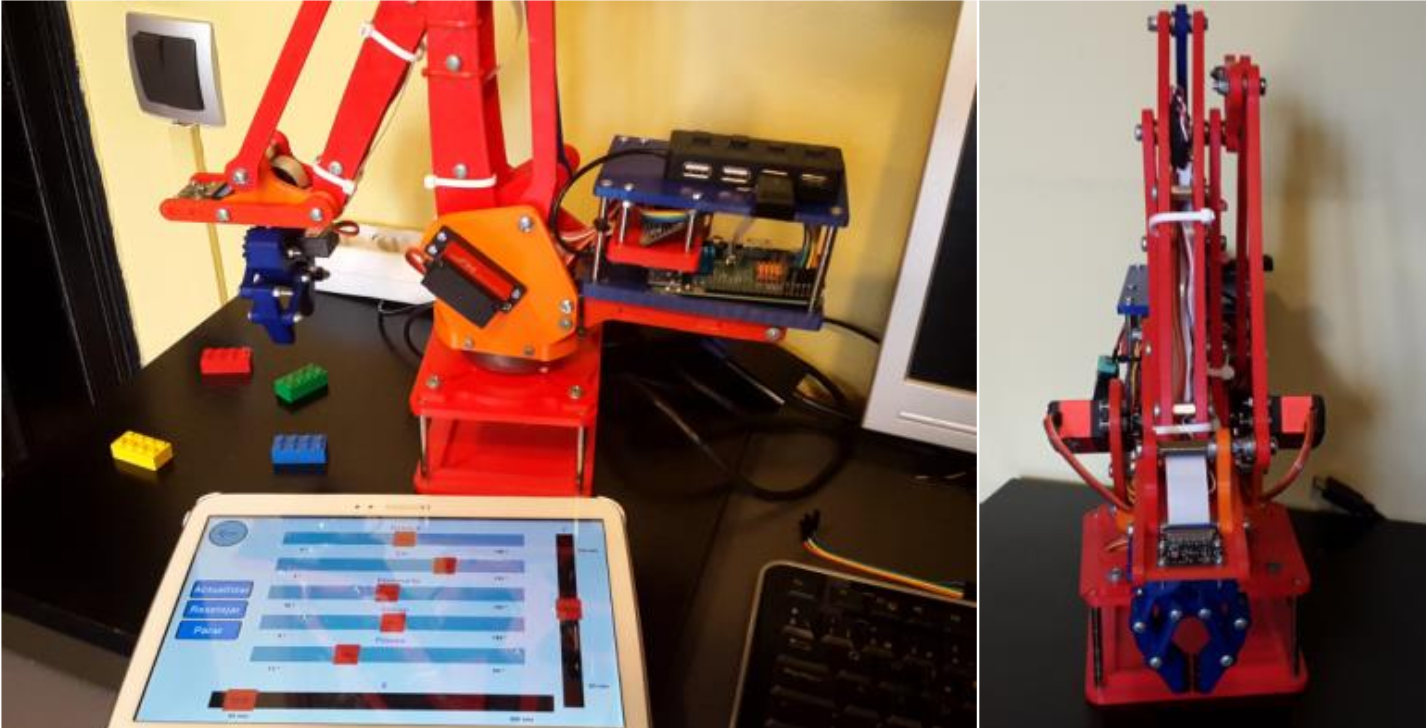
\includegraphics[width = .6\textwidth]{Robot.png}
  \caption{Brazo robótico casero.}
  \label{fig:brazo_robotico}
\end{figure}

La idea inicial se basaba en que la Raspberry fuese el cerebro de una partida de
tres en raya con un humano. Es decir, que fuese la encargada de recoger el input
de un jugador, decidir donde mover su pieza (de forma inteligente), mover el
brazo para recoger las piezas correspondientes. Tras consultar la documentación
del brazo robótico se dedicaron 6 semanas para el desarrollo del código de
movimiento. \\

Una vez terminado y calibrado el robot se decidió a probarlo, advirtiendo un
problema que podría ser crucial. El servo encargado de levantar piezas
deslizaba, con lo que era imposible llevar al robot a una posición concreta. Con
la idea de solucionar este problema se desmontó parte del robot y cambió la
pieza problemática. No obstante, otro servo diferente empezó a fallar tras una
semana de uso para comprobaciones. Sin piezas de recambio y con la imposibilidad
de comprar servos nuevos debido a su coste elevado se decidió trasladar el
proyecto hacia una simulación.


% Motivación.
\subsection{Replanteamiento del proyecto}
Finalmente, el proyecto se definió como el desarrollo de un programa capaz de
jugar de manera inteligente al juego del Tres en Raya y realizar una simulación
de un robot moviendo las piezas. \\

El nuevo rol de la Raspberry Pi es ser el host del servidor donde correrá el
código, simulación, etc. Se podría decir que en vez de controlar un periférico
``real'', controla el estado de la simulación que no deja de ser una
interpretación de la realidad.


\subsection{Objetivos}
El producto final pretende ser una interfaz web donde el jugador pueda realizar
una partida contra la máquina (o máquina vs. jugador) y ver el progreso de la
partida en la simulación. \\

Sabiendo que el juego del tres en raya es un juego de suma cero (si se suman las
pérdidas y las ganancias dan 0) se puede evitar la derrota siempre que no se
realicen movimientos incorrectos. Por lo tanto, no solo se plantea la creación
de un programa ``inteligente'' que incluya una simulación, sino que se creará un
programa capaz de evitar perder siempre. \\

En cuanto a la simulación, debido a la complejidad de gráficos 3D se decidió
dividirla en dos planos; alzado y planta. De esta forma, no se compromete la
imagen espacial sin adentrarse en el mundo de simulaciones 3D. Uno de los
objetivos de la simulación es ser capaz de sincronizar los dos planos e integrar
la rotación en el alzado, es decir, que los objetos en el alzado desaparezcan
gradualmente a medida que rota la planta. \\

\begin{figure}[htbp]
  \centering
  \begin{subfigure}{.5\textwidth}
    \centering
    \href{https://alvarezrosa.com/proyecto/}{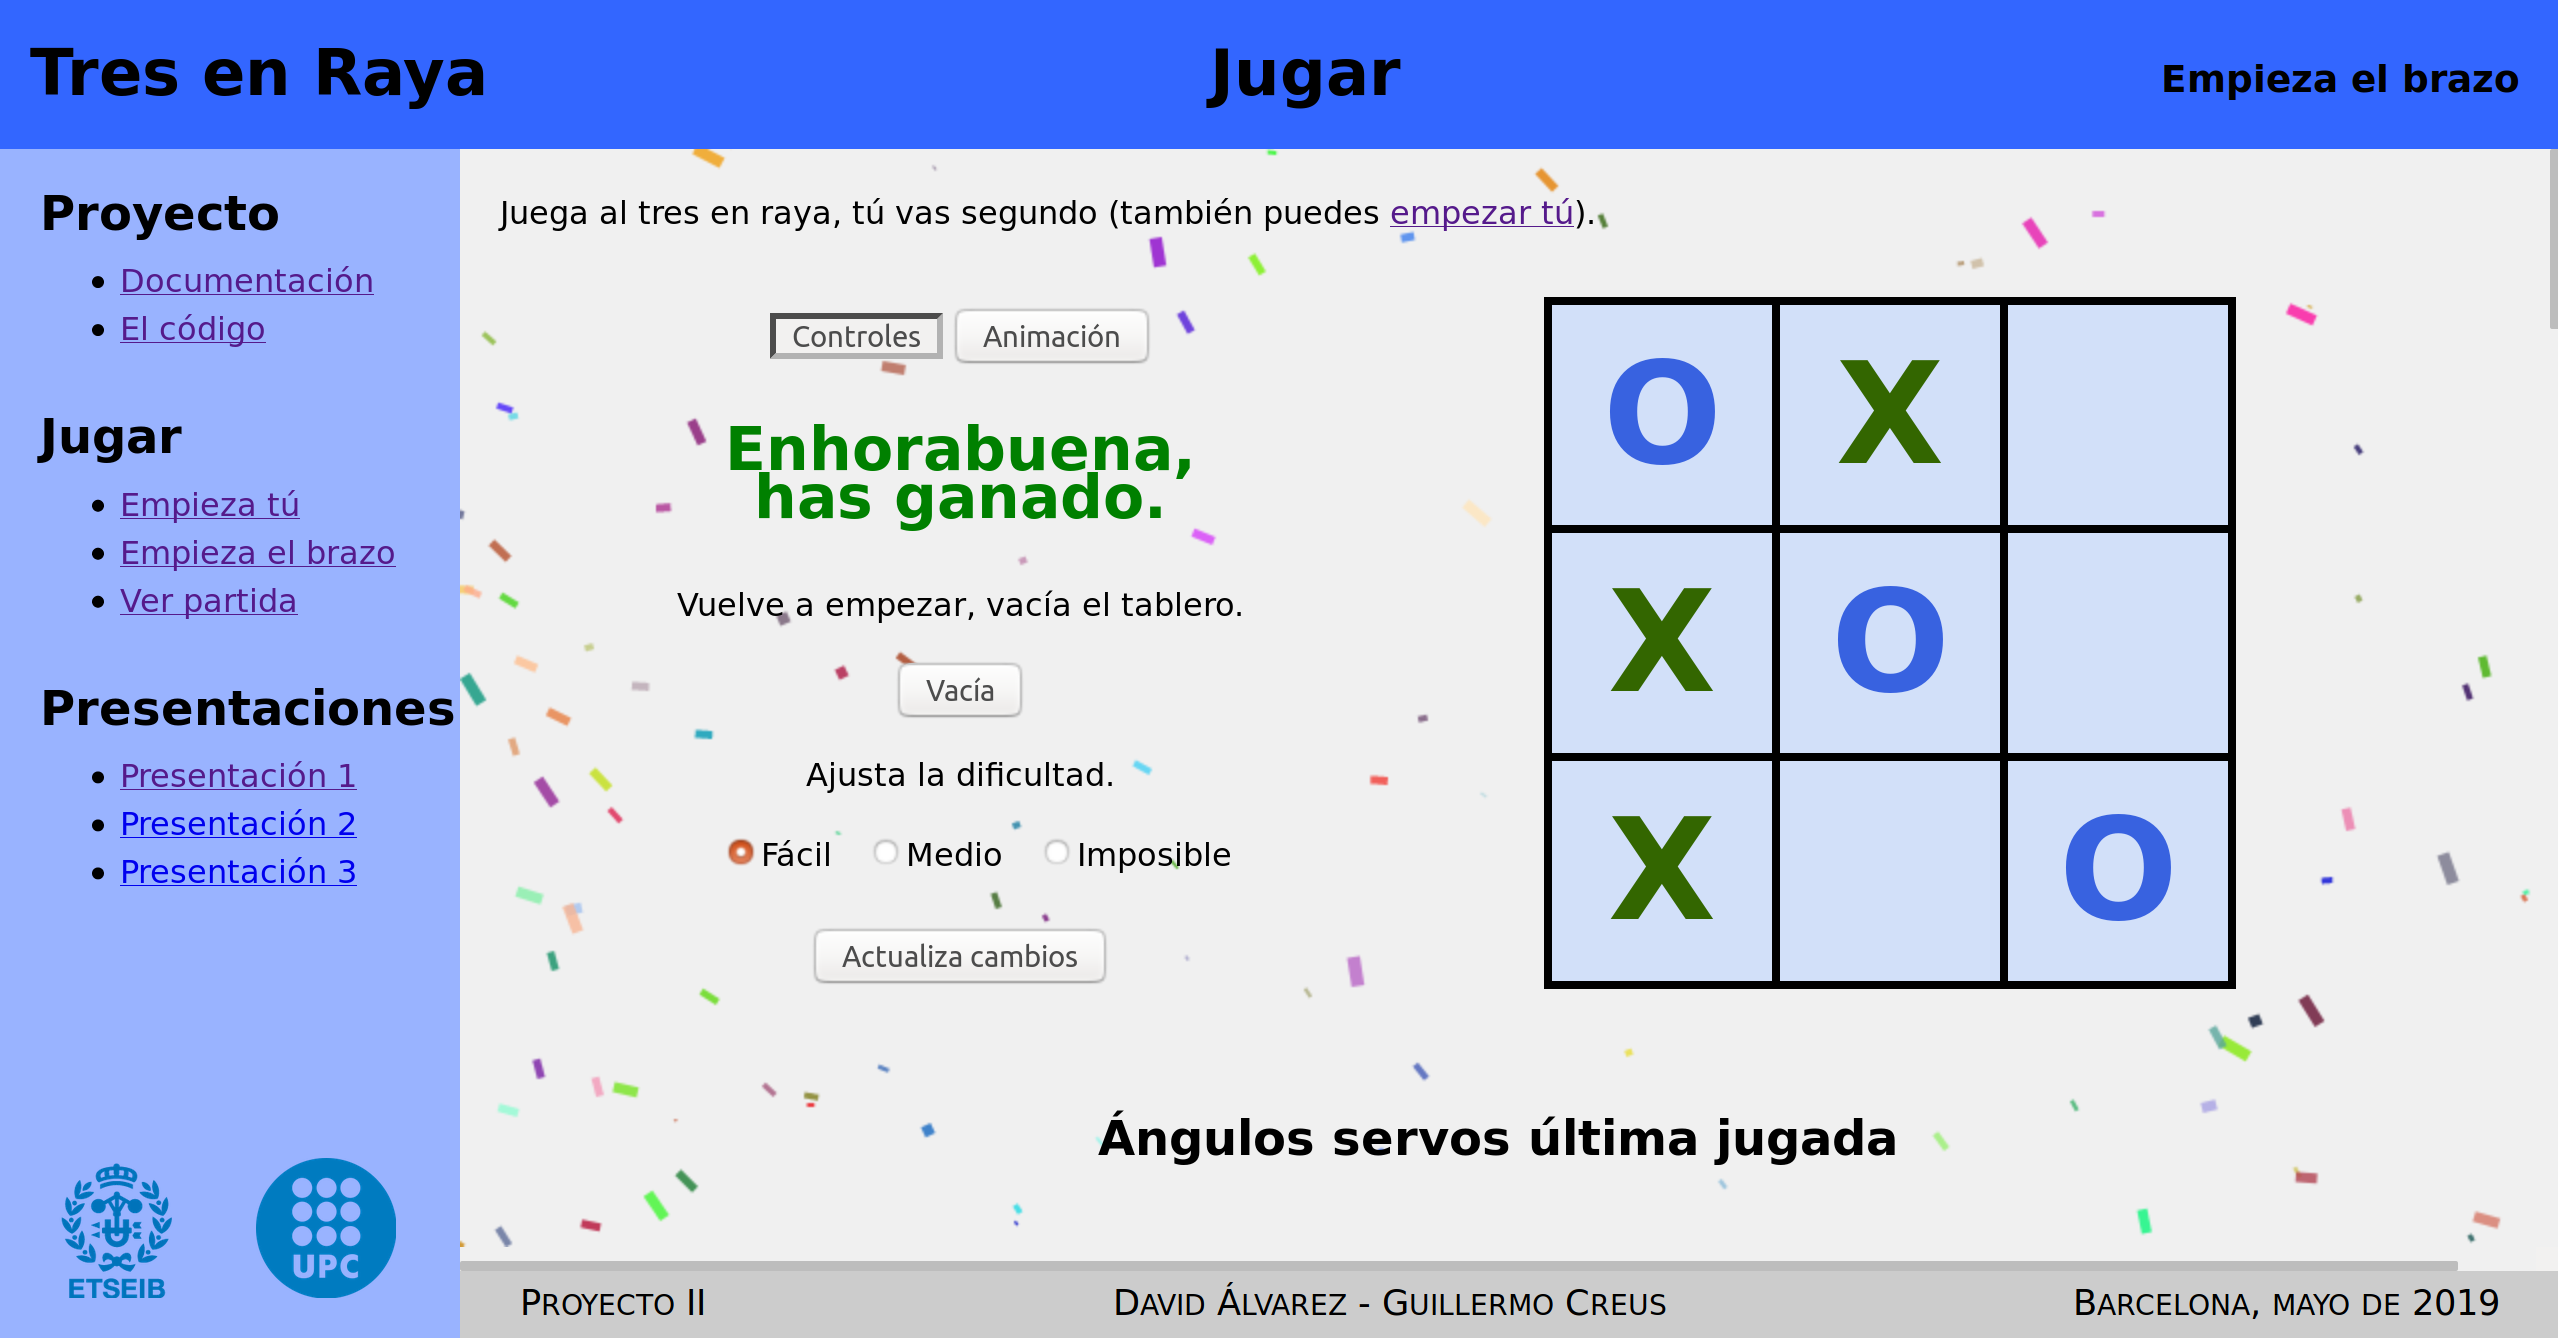
\includegraphics[width=.9\textwidth]{Interfaz_web.png}}
    \caption{Juego tres en raya interactivo.}
    \label{fig:sub1}
  \end{subfigure}%
  \begin{subfigure}{.5\textwidth}
    \centering
    \href{https://alvarezrosa.com/proyecto/}{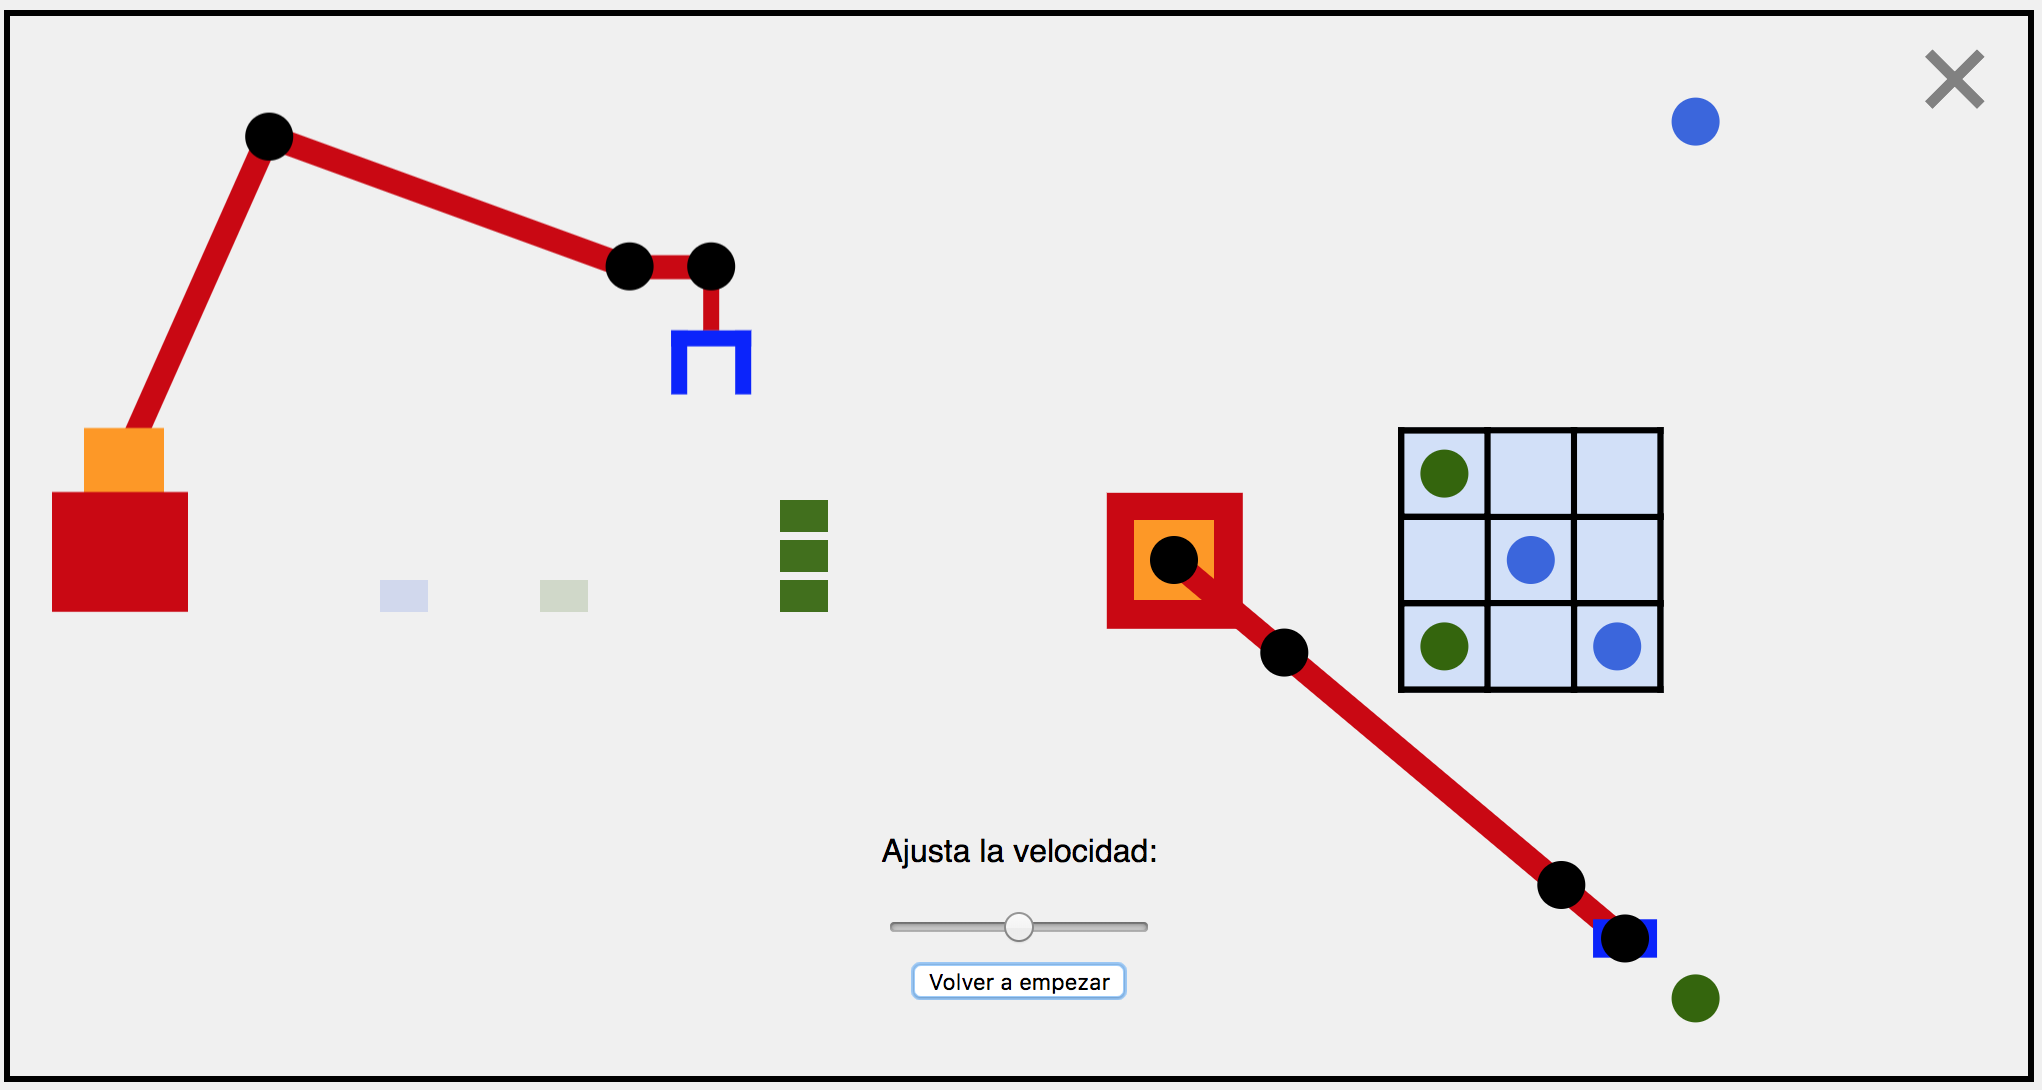
\includegraphics[width=.9\textwidth]{Animacion.png}}
    \caption{Simulación brazo robótico.}
    \label{fig:sub2}
  \end{subfigure}
  \caption{Interfaz Web.}
  \label{fig:test}
\end{figure}

\subsection{Alcance}
Una vez definido el objetivo del proyecto se procede al alcance del mismo:

\begin{itemize}
  \item Puesta en marcha de un servidor capaz de generar una interfaz web que
  recoja el input (jugada humano), genere un output adecuado (jugada AI) y lo
  plasme en una animación.
\end{itemize}

\section{Herramientas e implementación}

A continuación recogemos las herramientas informáticas usadas para desarrollar
este proyecto así como los diferentes lenguajes de programación que se han
usado.


\subsection{Tres en raya}

\begin{wrapfigure}{R}{.3\textwidth}
  \centering
  
\includegraphics[width = .15\textwidth]{Logo_Python.png}
  \caption{Lenguaje utilizado en el tres en raya.}
  \label{fig:python}
\end{wrapfigure}

Para desarrollar el tres en raya se han explorado manualmente todas las
posibilidades (exceptuando simetrías) y expresado en forma de árbol. A partir de
ahí, se ha trabajado en Python respetando la estructura definida
anteriormente. Es decir, Python sabe lo que hacer gracias a un árbol
implementado y lo único que debe hacer es bajar por las ramas correctas. Este
árbol está internamente en Python siguiendo como si fuera un grafo. Esto es,
consiste en una lista de nodos numerados y otras lista de conexiones entre
nodos. \\


\subsection{Interfaz gráfica}

Quisimos también ofrecer una interfaz gráfica en la que el usuario pudiese
interactuar con el proyecto. Donde se pudiera jugar al tres en raya de manera
sencilla y teniendo una respuesta mucho más visual del programa. Entre otras
opciones que se consideraron, se optó finalmente por una interfaz web debido a
que es un formato muy versátil y teníamos cierta experiencia anterior. \\

\begin{wrapfigure}{R}{.3\textwidth}
  \centering
  \hfill
  
\includegraphics[width = .25\textwidth]{Logo_Apache.png}
  \caption{Servidor Web Apache.}
  \label{fig:apache}
\end{wrapfigure}

Para poder hacer funcionar la web es necesario un servidor. En nuestro caso nos
decidimos por el servidor web \href{https://httpd.apache.org/}{Apache}. Se hizo
esta elección teniendo en cuenta que es software libre y que es el servidor más
usado en el mundo. Se configuró correctamente para poder funcionar con PHP
\imgInline{Logo_PHP.png} y que éste pudiera ejecutar código en Python
\imgInline{Logo_Python.png}  \\

Se está usando el lenguaje PHP como un enlace entre la web y el código de
Python. Es decir, PHP es el que se encarga de ejecutar el código de Python en el
servidor web con los parámetros adecuados dependiendo de la petición del
usuario. Cuando el usuario interactúa con la web realizando algún movimiento en
el tablero, es el código en PHP el que se encarga de transmitir este nuevo
movimiento (junto con los anteriores) al código de Python para que este de un
movimiento respuesta y mueva los servomotores a los ángulos adecuados. Por
último es también PHP el que se encarga de construir la web (con la nueva
información devuelta por Python) y así mostrársela al usuario. \\

Este funcionamiento global se encuentra recogido de manera esquemática en la
figura \vref{fig:arquitectura}.

\begin{figure}[p]
  \centering
  % -*- TeX-master: "Informe.tex" -*-

\begin{tikzpicture}
  % Cliente.
  \node[boxp = magenta] (Us) {Usuario};
  \node[box = magenta] (UN) [right = of Us] {Navegador};
  \begin{scope}[on background layer]
    \node[fit = (Us)(UN), cont = magenta, label = {Cliente}] (U) {};
  \end{scope}

  % Servidor Web.
  \node[boxp = gray] (SI) [below = 1.25 of U, xshift = -6.5] {\textit{Index}};
  \node[box = gray] (ST) [left = .75 of SI] {Tablero};
  \node[box = gray] (SN) [right = .75 of SI] {\textit{Navbar}};
  \node[box = gray] (SD) [below = .5 of ST] {Data};
  \node[box = gray] (SA) [right = .35 of SD] {Animación};
  \node[box = gray] (SC) [below = .5 of SN] {Controles};
  \node[box = gray] (SCi) [below = .5 of SD] {Animación};
  \node[box = gray] (SF) [below = .5 of SA, xshift = .25cm] {\textit{Footer}};
  \node[box = gray] (SE) [below = .5 of SC, xshift = .55cm] {Otros \ldots};
  \begin{scope}[on background layer]
    \node[fit = (SI)(ST)(SN)(SC)(SCi)(SD)(SE)(SA), cont = gray,
    label = above right:{Servidor Web}] (S) {};
  \end{scope}

  % Programa Principal.
  \node[boxp = orange] (Mai) [below = 1.5 of S] {Main};
  \begin{scope}[on background layer]
    \node[fit = (Mai), cont = orange, label = below:{Programa principal}] (Ma) {};
  \end{scope}

  % Brazo robótico.
  \node[boxp = red] (MM) [above right = .25 and 4 of Ma] {Principal};
  \node[box = red] (MP) [below = .5 of MM] {Plano};
  \node[box = red] (MI) [below = .5 of MP] {Interpolación};
  \begin{scope}[on background layer]
    \node[fit = (MM)(MP)(MI), cont = red, label = {Movimiento robot}] (M) {};
  \end{scope}

  % Tres en Raya.
  \node[boxp = blue] (TEs) [above left = .78 and 4 of Ma] {Principal};
  \node[box = blue] (TB) [below = .5 of TEs] {Básica};
  \node[box = blue] (TEq) [below = .5 of TB] {Equivalencias};
  \node[box = blue] (TA) [below = .5 of TEq] {Auxiliar};
  \begin{scope}[on background layer]
    \node[fit = (TEs)(TB)(TEq)(TA), cont = blue, label = {Estrategia Tres en Raya}] (T) {};
  \end{scope}

  % Conexiones globales.
  \connectV{U}{S};
  \connectV{S}{Ma};
  \connectH{T}{Ma};
  \connectH{Ma}{M};
\end{tikzpicture}

  \caption{Arquitectura del programa.}
  \label{fig:arquitectura}
\end{figure}


\subsection{Animación}

Para la simulación se han usado principalmente tres herramientas: \\

\begin{figure}[H]
  \centering
  
\includegraphics[width = .15\textwidth]{Logo_HTML.png}
  \hspace{1cm}
  
\includegraphics[width = .15\textwidth]{Logo_CSS.png}
  \hspace{1cm}
  
\includegraphics[width = .15\textwidth]{Logo_JS.png}
  \caption{Herramientas utilizadas en la simulación.}
  \label{fig:herramientas_simulacion}
\end{figure}

A grandes tiros, \textit{Hypertext Markup Language} (HTML) permite crear
webs. En este caso, HTML proporciona el espacio donde se realizará la
simulación. \textit{Cascading Style Sheets} (CSS) es el lenguaje utilizado para
modificar la presentación de un documento HTML. CSS es la herramienta que ha
permitido crear las figuras y determinar la disposición en el HTML. Por último,
\textit{JavaScript} es el lenguaje de programación que ha permitido modificar el
CSS. En otras palabras, al modificar la presentación del documento HTML se crea
la simulación.


\section{Funcionamiento}

A continuación se explicará el funcionamiento y la lógica detrás de este
proyecto, que se encarga de decidir el siguiente movimiento (estrategia del tres
en raya) y de animar el robot virtual desarrollado.


\subsection{Tres en Raya}

Como se ha comentado anteriormente no solo se pretendía crear un jugador al 3 en
raya, sino que fuese invencible. Esto es posible debido a la condición de ser un
juego de suma cero, ya que nos permite desarrollar las ramas posibles antes y
evitar aquellas que beneficien al oponente (y obviamente guiar al jugador a la
derrota). \\

Realizar lo mencionado no es tan sencillo como parece. Aunque sea un juego con
pocas posibilidades respecto a otros como el ajedrez, GO, etc. cuenta con $9! =
362.880$ posibilidades (9 casillas al principio, 8 en la siguiente tirada
\ldots). Para cualquier dispositivo sería una carga extra que se debería
optimizar. La propuesta para este trabajo es crear un programa en Python que
conozca todas los casos base (exceptuando simetrías) y extrapole a los otros
respuestas mediante simetrías. Por ejemplo, si se desea saber cual es la jugada
óptima si la primera jugada toca en un extremo se explorará la rama y se
escogerá una rama en la que el jugador no pueda ganar. En este caso, como se ve
en la figura \ref{fig:rama}, la jugada óptima tocaría en el medio.\\

\begin{figure}[htbp]
  \centering
  \scalebox{.5}{% -*- TeX-master: "Informe.tex" -*-

\begin{tikzpicture}[tree]
  \node[board] {
    \o \& \e \& \e \\
    \e \& \e \& \e \\
    \e \& \e \& \e \\
  }
  child {
    node[board] {
      \o \& \e \& \e \\
      \e \& \x \& \e \\
      \e \& \e \& \e \\
    }
    child {
      node[board] {
        \o \& \o \& \e \\
        \e \& \x \& \e \\
        \e \& \e \& \e \\
      }
      \EB
    }
    child {
      node[board] {
        \o \& \e \& \o \\
        \e \& \x \& \e \\
        \e \& \e \& \e \\
      }
      \EB
    }
    child {
      node[board] {
        \o \& \e \& \e \\
        \e \& \x \& \o \\
        \e \& \e \& \e \\
      }
      child{
        node[board] {
          \o \& \e \& \e \\
          \e \& \x \& \o \\
          \x \& \e \& \e \\
        }
      }
      \EB
    }
    child {
      node[board] {
        \o \& \e \& \e \\
        \e \& \x \& \e \\
        \e \& \e \& \o \\
      }
      child {
        node[board] {
          \o \& \x \& \e \\
          \e \& \x \& \e \\
          \e \& \e \& \o \\
        }
      }
      \EB
    }
  };
\end{tikzpicture}
}
  \caption{Una rama como ejemplo.}
  \label{fig:rama}
\end{figure}

A partir de esta jugada se diferencian cuatro posibilidades del oponente. Para
cada posibilidad se explorará el árbol y se decidirá que jugada interesa. Como
el tablero se va llenando, llegará un punto en el que la partida sea tablas o se
ha forzado la victoria mediante un jaque. En este momento, se despliega la
estrategia básica que consiste en lo siguiente:

\begin{enumerate}
  \item Comprueba si podemos ganar:
  \begin{enumerate}
    \item PUEDO: juega y gana
    \item NO PUEDO: siguiente
  \end{enumerate}
  \item Comprueba si podemos perder:
  \begin{enumerate}
    \item PUEDO: tapo la posibilidad y sigo jugando
    \item NO PUEDO: jugada aleatoria
  \end{enumerate}
\end{enumerate}

Una vez definido el algoritmo para jugar uno se pregunta, ¿Se debe repetir el
proceso de encontrar la rama si el jugador en vez de tirar al extremo superior
izquierdo lo hace en el derecho? La respuesta de un humano sería claramente no,
ya que sabe que existe una simetría respecto el eje $y$, con lo que extrapolaría
los resultados obtenidos anteriormente. \\

\begin{figure}[htbp]
  \centering
  \scalebox{.35}{% -*- TeX-master: "Presentación.tex" -*-


% Simetrías.

\begin{tikzpicture}
  \node[board, draw] (R) {
    \x \& \e \& \e \\
    \e \& \e \& \e \\
    \e \& \e \& \e \\
  };
  \node[board, right = of R] (A) {
    \x \& \o \& \e \\
    \e \& \e \& \e \\
    \e \& \e \& \e \\
  };
  \node[board, right = of A] (B) {
    \x \& \e \& \o \\
    \e \& \e \& \e \\
    \e \& \e \& \e \\
  };
  \node[board, below = of R] (C) {
    \x \& \e \& \e \\
    \o \& \e \& \e \\
    \e \& \e \& \e \\
  };
  \node[board, below = of A] (D) {
    \x \& \e \& \e \\
    \e \& \o \& \e \\
    \e \& \e \& \e \\
  };
  \node[board, below = of B] (E) {
    \x \& \e \& \e \\
    \e \& \e \& \o \\
    \e \& \e \& \e \\
  };
  \node[board, below = of C] (F) {
    \x \& \e \& \e \\
    \e \& \e \& \e \\
    \o \& \e \& \e \\
  };
  \node[board, below = of D] (G) {
    \x \& \e \& \e \\
    \e \& \e \& \e \\
    \e \& \o \& \e \\
  };
  \node[board, below = of E] (H) {
    \x \& \e \& \e \\
    \e \& \e \& \e \\
    \e \& \e \& \o \\
  };
  \pause
  \draw[<->, ultra thick] (A-3-1.south west) to node[right]{Simetría}
  (C-1-3.north east);
  \draw[<->, ultra thick] (B-3-1.south west) to node[right, very near
  start]{Simetría} (F-1-3.north east);
  \draw[<->, ultra thick] (E-3-1.south west) to node[right]{Simetría}
  (G-1-3.north east);
  \cross{C}
  \cross{F}
  \cross{G}
\end{tikzpicture}
}
  \hspace{1cm}
  \scalebox{.35}{% -*- TeX-master: "Informe.tex" -*-


\begin{tikzpicture}
  \node[board, draw] (R) {
    \x \& \e \& \e \\
    \e \& \e \& \e \\
    \e \& \e \& \e \\
  };
  \node[board, right = of R] (A) {
    \x \& \o \& \e \\
    \e \& \e \& \e \\
    \e \& \e \& \e \\
  };
  \node[board, right = of A] (B) {
    \x \& \e \& \o \\
    \e \& \e \& \e \\
    \e \& \e \& \e \\
  };
  \node[board, below = of R] (C) {
    \x \& \e \& \e \\
    \o \& \e \& \e \\
    \e \& \e \& \e \\
  };
  \node[board, below = of A] (D) {
    \x \& \e \& \e \\
    \e \& \o \& \e \\
    \e \& \e \& \e \\
  };
  \node[board, below = of B] (E) {
    \x \& \e \& \e \\
    \e \& \e \& \o \\
    \e \& \e \& \e \\
  };
  \node[board, below = of C] (F) {
    \x \& \e \& \e \\
    \e \& \e \& \e \\
    \o \& \e \& \e \\
  };
  \node[board, below = of D] (G) {
    \x \& \e \& \e \\
    \e \& \e \& \e \\
    \e \& \o \& \e \\
  };
  \node[board, below = of E] (H) {
    \x \& \e \& \e \\
    \e \& \e \& \e \\
    \e \& \e \& \o \\
  };
  \draw[unir] (A-3-1.south west) to node[right] {Simetría} (C-1-3.north east);
  \draw[unir] (B-3-1.south west) to node[right, very near start] {Simetría}
  (F-1-3.north east);
  \draw[unir] (E-3-1.south west) to node[right]{Simetría} (G-1-3.north east);
\end{tikzpicture}
}
  \hspace{1cm}
  \scalebox{.35}{% -*- TeX-master: "Informe.tex" -*-


\begin{tikzpicture}
  \node[board, draw] (R) {
    \x \& \e \& \e \\
    \e \& \e \& \e \\
    \e \& \e \& \e \\
  };
  \node[board, right = of R] (A) {
    \x \& \o \& \e \\
    \e \& \e \& \e \\
    \e \& \e \& \e \\
  };
  \node[board, right = of A] (B) {
    \x \& \e \& \o \\
    \e \& \e \& \e \\
    \e \& \e \& \e \\
  };
  \node[board, below = of R] (C) {
    \x \& \e \& \e \\
    \o \& \e \& \e \\
    \e \& \e \& \e \\
  };
  \node[board, below = of A] (D) {
    \x \& \e \& \e \\
    \e \& \o \& \e \\
    \e \& \e \& \e \\
  };
  \node[board, below = of B] (E) {
    \x \& \e \& \e \\
    \e \& \e \& \o \\
    \e \& \e \& \e \\
  };
  \node[board, below = of C] (F) {
    \x \& \e \& \e \\
    \e \& \e \& \e \\
    \o \& \e \& \e \\
  };
  \node[board, below = of D] (G) {
    \x \& \e \& \e \\
    \e \& \e \& \e \\
    \e \& \o \& \e \\
  };
  \node[board, below = of E] (H) {
    \x \& \e \& \e \\
    \e \& \e \& \e \\
    \e \& \e \& \o \\
  };
  \draw[unir] (A-3-1.south west) to node[right] {Simetría} (C-1-3.north east);
  \draw[unir] (B-3-1.south west) to node[right, very near start] {Simetría}
  (F-1-3.north east);
  \draw[unir] (E-3-1.south west) to node[right]{Simetría} (G-1-3.north east);
  \cross{C}
  \cross{F}
  \cross{G}
\end{tikzpicture}
}
  \caption{Tableros simétricos equivalentes.}
  \label{fig:simetrias}
\end{figure}

La esencia del algoritmo se basa en las ramas desarrolladas y en las
simetrías. El ordenador trabaja con un tablero interno y en cada jugada
identifica la simetría que induce ese movimiento. Nótese que solo existen 5
simetrías:

\begin{enumerate}
  \item Identidad.
  \item Eje x.
  \item Eje y.
  \item Diagonal 1.
  \item Diagonal 2.
\end{enumerate}

Esta simetría se guarda en el vector de simetrías y cada vez que quiere traducir
algún resultado le aplica el vector de simetrías (Composición de simetrías $\equiv$
simetría).

\subsection{Movimiento}

Para el movimiento se han definido dos planos de actuación: planta y
alzado. Esta simplificación respecto a la simulación 3D implica que la planta y
el alzado deben ir sincronizados. \\

\begin{figure}[htbp]
  \centering
  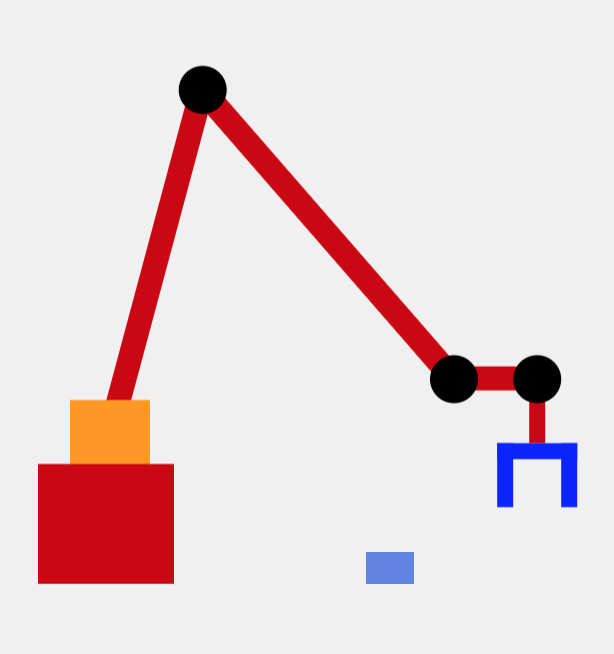
\includegraphics[width = .3\textwidth]{Brazo_escala.png}
  \hspace{1.5cm}
  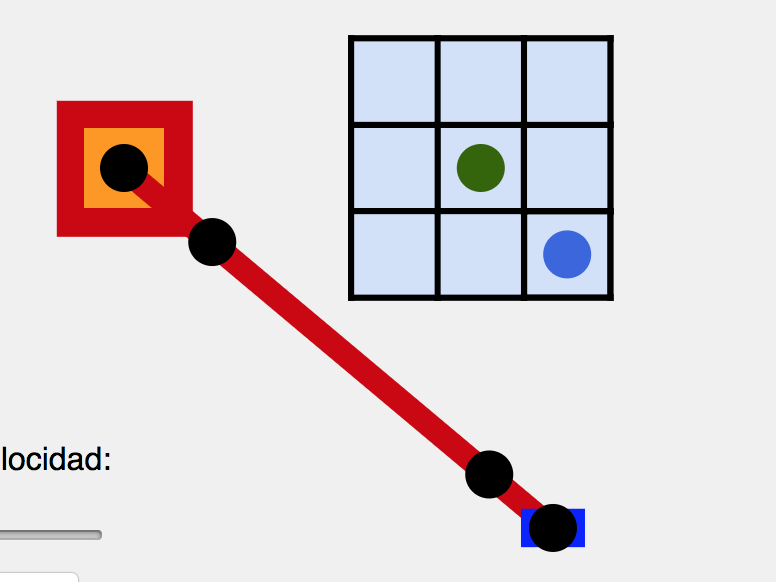
\includegraphics[width = .3\textwidth]{Planta_robot_escala.png}
  \caption{Brazo robótico a escala}
  \label{fig:brazo_escala}
\end{figure}

Se ha utilizado un modelo a escala del brazo de la figura
\ref{fig:brazo_robotico} (en la página \pageref{fig:brazo_robotico}) mediante
CSS. Se ha definido cada elemento por separado y se han ido uniendo mediante
``containers'' (para poder mover varios elementos a la vez). \\

El hecho que sea a escala implica que la simulación sea más realista y los
ángulos de movimientos se pueden reciclar del programa creado para el movimiento
del brazo real. El funcionamiento de la simulación del alzado es relativamente
sencilla (una vez creados los subprogramas):

\begin{enumerate}
  \item Se definen los puntos del espacio donde se encuentran los almacenes de
  piezas y el tablero.
  \item Mediante resolución analítica de las ecuaciones de enlace calcula los
  ángulos necesarios para orientar las barras y poder coger la pieza.
  \item Llama a la función de JS encargada de mover las barras a los ángulos
  calculados.
  \item Calcula los ángulos para dejar la pieza en el tablero.
  \item Mismo que en (2).
\end{enumerate}

Para añadir la simulación de la planta lo único que hay que añadir es una
función que acorte la longitud de las barras cuando roten las barras del
alzado. Esto se consigue calculando proyecciones respecto al eje x.


\section{Planificación y costes}

La planificación del proyecto se ha dividido de la siguiente manera:

\begin{outline}
  \1 12 Febrero - 26 Febrero:
  \2 Definición del proyecto.
  \3 Investigación librerías servos. \\

  \1 26 Febrero - 23 Abril
  \2 Robot.
  \3 Código movimiento.
  \3 Pruebas movimiento.
  \3 Reparación.
  \2 3 en raya.
  \3 Desarrollo árbol de posibilidades.
  \3 Implementación en Python.
  \2 Diseño Web.
  \3 Creación HTML/CSS Tablero.
\end{outline}

A partir de este momento se decide realizar la simulación:

\begin{outline}
  \1 23 Abril -21 Mayo
  \2 Simulación
  \2 Servidor
\end{outline}

El desarrollo de este proyecto ha requerido diferentes lenguajes de
programación, en la tabla \ref{tab:lineas} se resumen el número de líneas de
código por lenguaje de programación y el número de archivos.

\begin{table}[htbp]
  \centering
  \renewcommand{\arraystretch}{1.25}
  \setlength{\tabcolsep}{1.5\tabcolsep}
  \rowcolors{2}{white}{gray!30}
  \caption{Líneas de código y número de archivos.}
  \label{tab:lineas}
  \begin{tabular}{*3c}
    \toprule
    Lenguaje & \# Archivos & \# Líneas total \\
    \midrule
    Python \imgInline{Logo_Python.png} & 9 & 1025 \\
    JavaScript \imgInline{Logo_JS.png} & 2 & 366 \\
    PHP \imgInline{Logo_PHP.png} + HTML \imgInline{Logo_HTML.png} & 18 & 1315 \\
    CSS \imgInline{Logo_CSS.png} & 3 & 696 \\
    \hline
    TOTAL & 32 & 3402 \\
    \bottomrule
  \end{tabular}
\end{table}

Este número de lineas ha sido calculado de manera sencilla usando tuberías en la
terminal. Por ejemplo, para contar el número de líneas de código que hay entre
HTML y PHP en el servidor web se puede hacer:

\begin{verbatim}
$ cat Servidor\ Web/**/*.{html,php} | wc -l
\end{verbatim}

Donde se ha usado el programa \verb|cat| que imprime por terminal el contenido
de un archivo y se le pasa este output mediante una tubería al programa
\verb|wc| que se encarga de contar el número de líneas. De manera similar,
para contar el número de archivos escritos, por ejemplo, en Python, se puede hacer:

\begin{verbatim}
$ ls -l Servidor\ Web/**/*.py | wc -l
\end{verbatim}

- \underline{Nota}: Estos comandos podrian fallar si no está activa la
funcionalidad de \verb|**| en la terminal, esto se puede hacer (en Bash al
menos) con el comando \verb|shopt -s globstar|. \\

A continuación se presentan en la tabla \ref{tab:costes} los costes del proyecto
suponiendo que una empresa interesada en el ámbito encargase un proyecto similar
al realizado:

\begin{table}[htbp]
  \centering
  \renewcommand{\arraystretch}{1.25}
  \setlength{\tabcolsep}{1.5\tabcolsep}
  \rowcolors{2}{white}{gray!30}
  \caption{Costes del proyecto.}
  \label{tab:costes}
  \begin{tabular}{llll}
    \toprule
    Tarea                             & Duración (h)   & Precio/hora (€/h) & Precio (€) \\
    \midrule
    Desarrollo de código en clase     & $2 \cdot (13 \cdot 2)$ & 20                & 1040       \\
    3 en raya (árbol)                 & 4              & 20                & 80         \\
    Código 3 en raya (implementación) & $2 \cdot 6$        & 20                & 240        \\
    Investigación librerías Servos    & 2              & 20                & 40         \\
    Código movimiento (robot real)    & $2 \cdot 14$       & 20                & 560        \\
    Reparación robot                  & 2              & 20                & 40         \\
    Simulación                        & $2 \cdot 14$       & 30                & 840        \\
    Creación Diseño Web               & 5              & 30                & 150        \\
    Puesta en marcha servidor         & 10             & 30                & 300        \\
    \hline
    TOTAL                             & 144            &                   & 3290       \\
    \bottomrule
  \end{tabular}
\end{table}


\section{Resultados y conclusiones}

El proyecto, como se ha ido exponiendo a lo largo del trabajo ha migrado de la
realidad a la web. Aunque la web no sea accesible a no ser que la Raspberry esté encendida y conectada a la red local, se puede acceder a ella mediante la web: \href{www.alvarezrosa.com/proyecto}{www.alvarezrosa.com/proyecto} . En esta web se encontrará todo lo relacionado con este proyecto, por ejemplo, en la pestaña ``Documentación'' se encuentra una copia de este informe en pdf y el código fuente (ya que ha sido
desarrollado en \LaTeX). \\

Para empezar a jugar se debe pinchar en ``Empieza tú'' o ``Empieza el brazo''
dependiendo de la modalidad de juego. Una vez dentro en la parte superior
aparecen dos botones: ``Controles'' y ``Simulación''. Para ver el tablero pinchará en la primera opción. En este pantalla se puede configurar la
dificultad del juego: ``Fácil'' (movimientos aleatorios), ``Medio'' (movimientos
evitando la derrota e intentando ganar pero puede perder) e ``Imposible'' (nunca
pierde). \\

Una vez introducida la jugada deseada, se podrá ver cómo mueve el robot
pinchando en el botón ``Simulación''. Se puede ver un ejemplo de simulación en
la figura \ref{fig:test} (en la página \pageref{fig:test}). Como cabe esperar,
la simulación muestra el movimiento del jugador seguido del de la máquina, es
decir, un turno completo. \\

\begin{figure}[htbp]
  \centering
  \href{https://alvarezrosa.com/proyecto/}{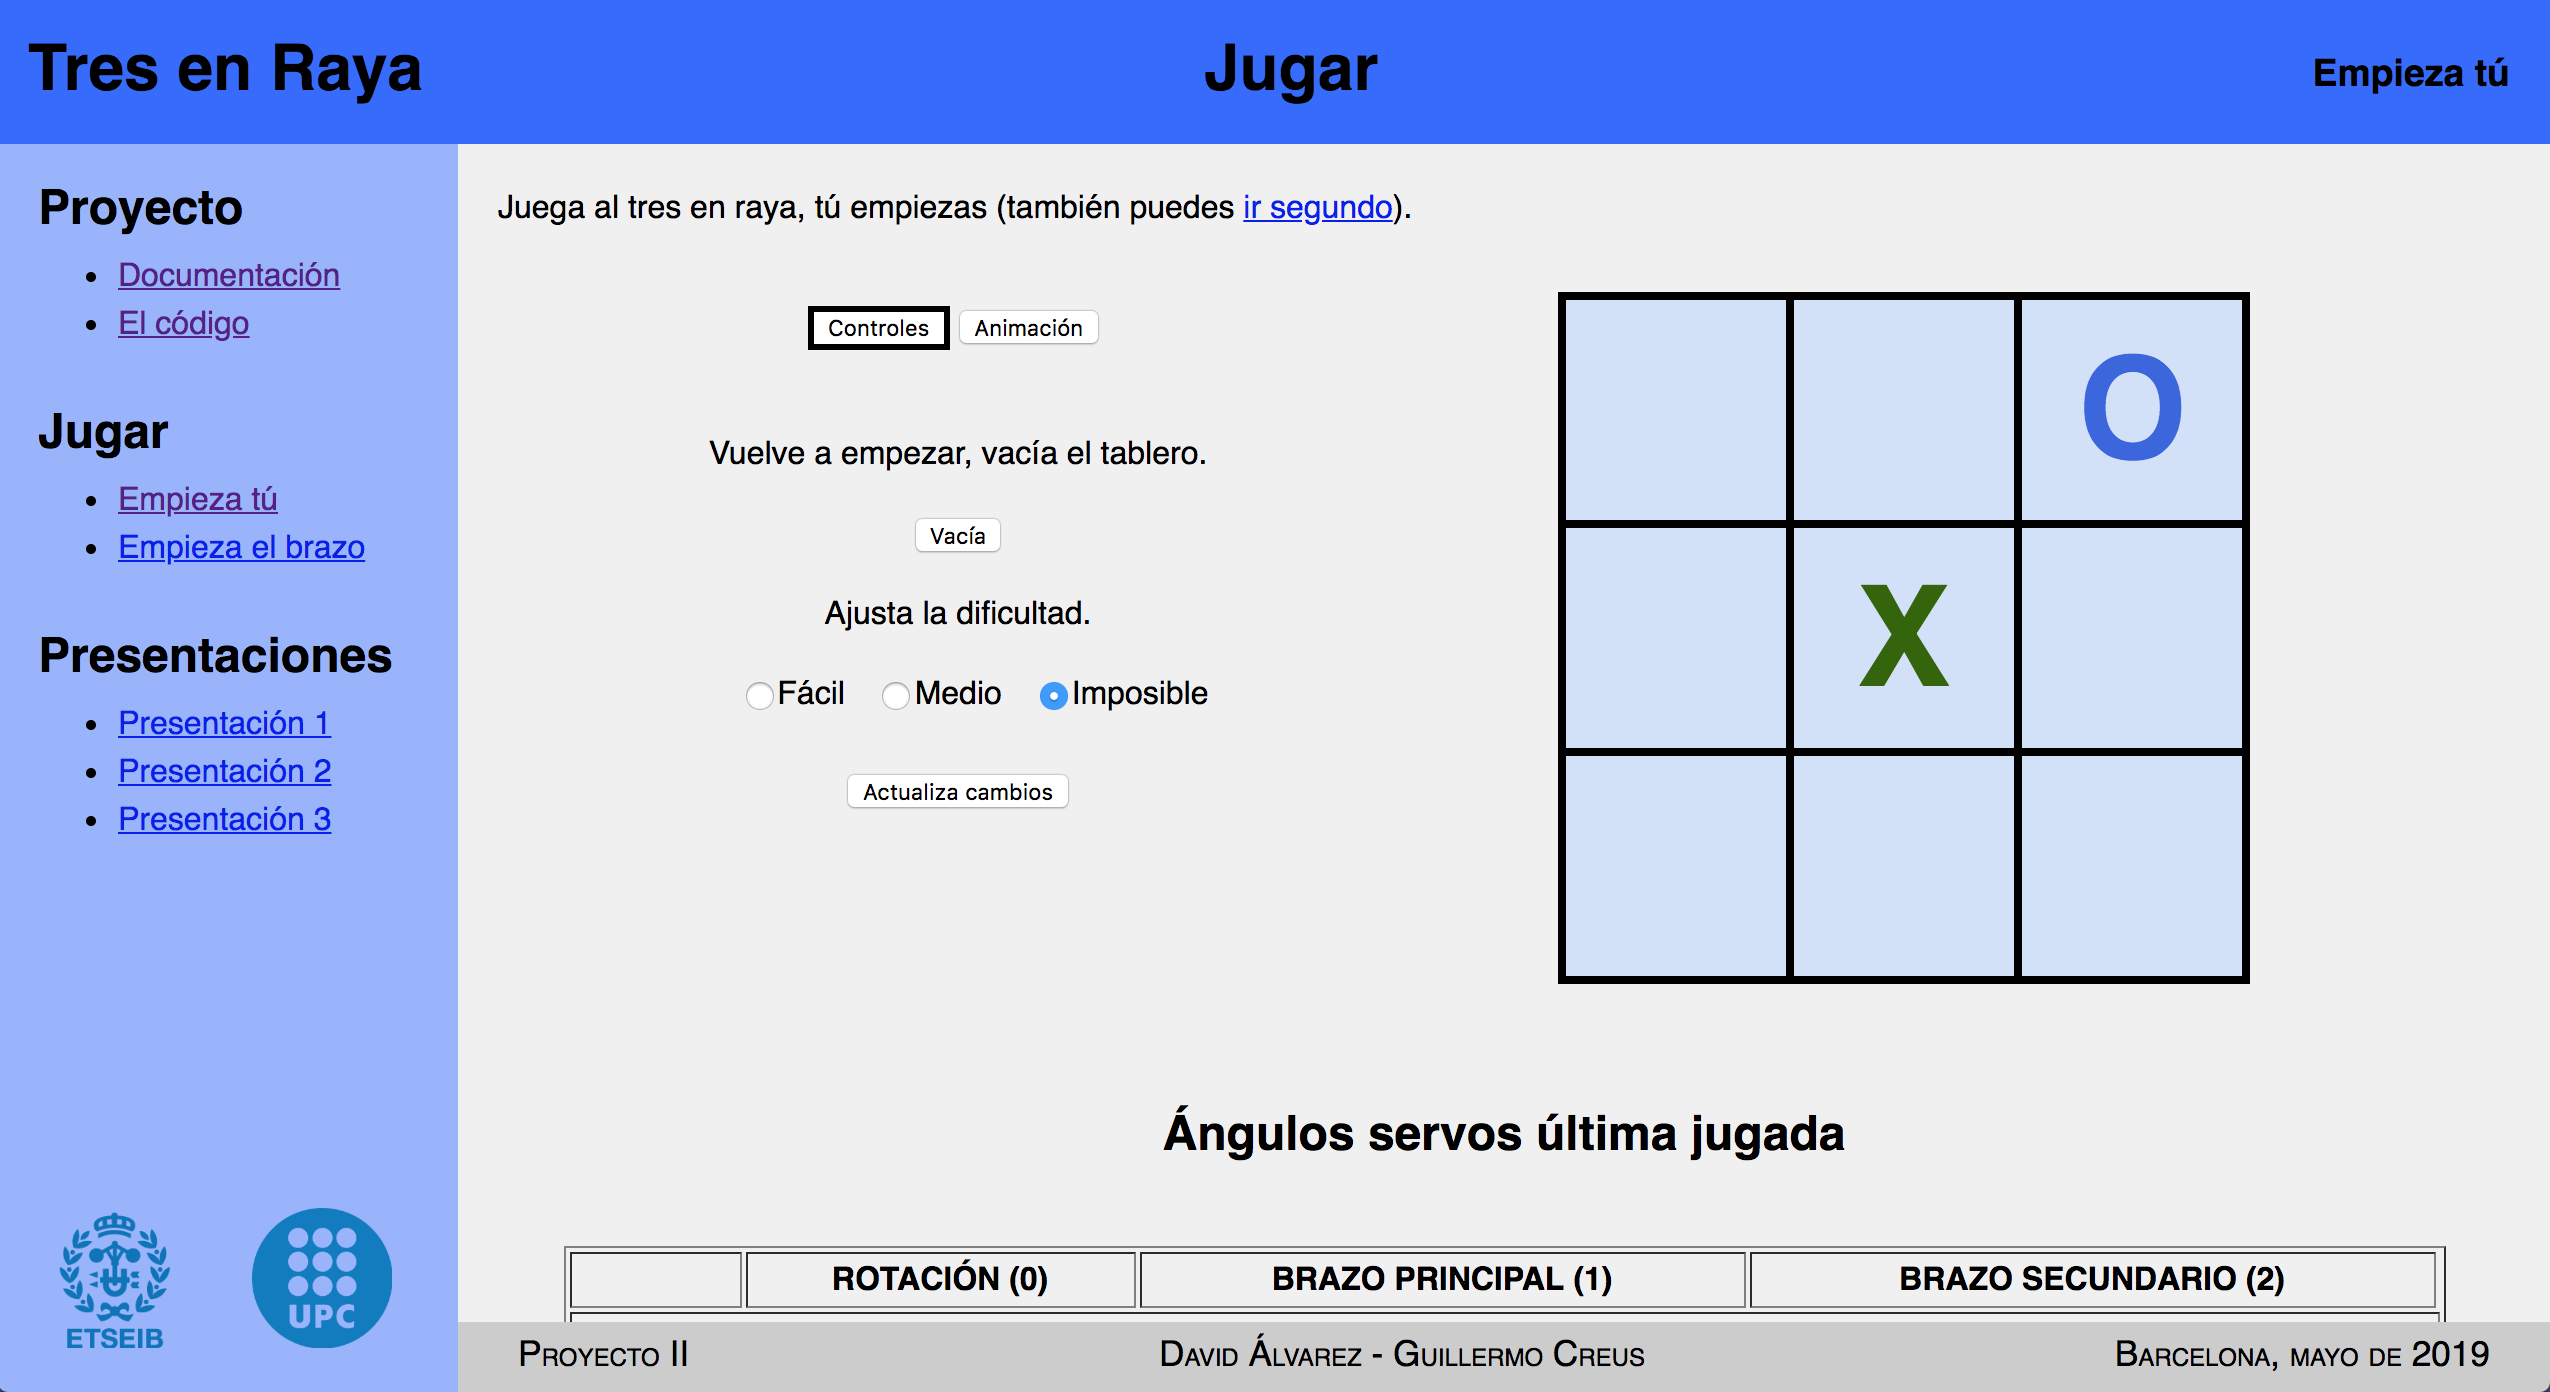
\includegraphics[width = 150mm]{Resultado_final.png}}
  \caption{Web - Resultado final}
  \label{fig:web_res_final}
\end{figure}

En cuanto a conclusiones se debe recalcar dos lecciones importantes que se han
aprendido a lo largo del proyecto. La primera es la dificultad de realizar
proyectos con elementos reales. Esto se aplica al proyecto ya que por culpa de
una pieza que a gran escala parece insignificante no se ha podido realizar el
proyecto que se tenía en mente al principio de curso. Por falta de tiempo y
presupuesto las consecuencias han sido devastadoras para los objetivos
iniciales. En un ambiente laboral se podría encontrar una solución que no
comprometiese tanto los objetivos iniciales y tampoco generase unas pérdidas
importantes (como sería comprar repuestos nuevos a los servos o comprar servos nuevos). Esta alternativa se podría haber
gestado en forma de creación de una pieza metálica que sustituya la
defectuosa. Cabe destacar que esta opción fue estudiada personalmente pero fue
desechada por falta de contactos en la industria. \\

No obstante, queda claro que los proyectos con elementos reales (y no reales
también pero la resolución depende más de los individuos) generan unos problemas
importantes que deben ser solucionados para llevarlo a cabo. La capacidad de
resolución de problemas de la vida real es el pan de cada día del ingeniero y es
su deber saber sortear, en la medida de lo posible, los problemas que amenacen
las ideas/objetivos iniciales. \\

La segunda lección es la importancia de las simulaciones en la vida
ingenieril. Como se ha comentado anteriormente los problemas de la vida real
generan complicaciones grandes, desgaste del material, gasto energético,
etc. Proporcionar una simulación a escala, como se ha desarrollado en este
proyecto, es muy interesante de cara a realizar un proyecto ya que se reducen
mucho las horas de experimentación. Se puede comprobar todo en el programa de
ordenador y una vez funcione experimentar. \\

Por último, se debe mencionar que este proyecto se ha realizado con filosofía
código libre por lo que en la pestaña ``El código'' se encuentran todos los
scripts necesarios para correr la web, realizar simulaciones y emular lo
conseguido en este proyecto.


\pagebreak
\appendix
% -*- TeX-master: "Informe.tex" -*-


\section{Árbol de directorios}

A continuación se muestra en la figura \ref{fig:directorios} el árbol de
directorios del Servidor Web, con todos los diferentes archivos que se han
creado. \\

\begin{figure}[H]
  \centering
  \scalebox{.93}{% -*- TeX-master: "Informe.tex" -*-

\begin{minipage}{.4\textwidth}
  \dirtree{%
    .1 \myFolder{Servidor Web}.
    .2 \myFolder{cgi-bin}.
    .3 {* El contenido está $\longrightarrow$}.
    %
    .2 \myFolder{jugar}.
    .3 \myFolder{ai}.
    .4 \myPhp{index}.
    .3 \myFolder{per}.
    .4 \myPhp{index}.
    %
    .3 \myCss{animacion}.
    .3 \myPhp{animacion}.
    .3 \myJs{animacion}.
    .3 \myJs{confeti}.
    .3 \myPhp{controles}.
    .3 \myPhp{data}.
    .3 \myPhp{index}.
    .3 \myPhp{tablero}.
    %
    .2 \myFolder{presentaciones}.
    .3 \myPhp{index}.
    .3 \myFolder{p1}.
    .4 \myPhp{index}. .4 \myPdf{p1}. .4 \myZip{p1}.
    .3 \myFolder{p2}.
    .4 * Análogo a p1 $\uparrow$.
    % .4 \myPhp{index}. .4 \myPdf{p1}. .4 \myZip{p1}.
    .3 \myFolder{p3}.
    .4 * Análogo a p1 $\uparrow$.
    % .4 \myPhp{index}. .4 \myPdf{p1}. .4 \myZip{p1}.
    .3 \myPhp{index}.
    %
    .2 \myFolder{proyecto}.
    .3 \myFolder{codigo}. % TODO: Revisar esta carpeta.
    .4 \myPhp{index}. .4 \myZip{TresEnRaya}.
    .3 \myFolder{documentacion}. % TODO: Revisar esta carpeta.
    .4 \myPhp{index}. .4 \myPdf{documentacion}. .4 \myZip{documentacion}.
    .3 \myPhp{index}.
    %
    .2 \myHtml{footer}.
    .2 \myPhp{index}.
    .2 \myCss{layout}.
    .2 \myImg{logo\_ETSEIB} \imgInline{Logo_ETSEIB.png}.
    .2 \myImg{logo\_UPC} \imgInline{Logo_UPC.png}.
    .2 \myHtml{navbar}.
    .2 \myCss{tablero}.
  }
\end{minipage}
\hspace{2.25cm}
\begin{minipage}{.4\textwidth}
  \dirtree{%
    .1 \myFolder{cgi-bin}.
    .2 \myFolder{movimiento}.
    .3 \myPy{main}.
    .3 \myPy{plano}.
    .3 \myPy{servos}.
    .2 \myFolder{estrategia}.
    .3 \myPy{basica}.
    .3 \myPy{cfg}.
    .3 \myPy{equivalencias}.
    .3 \myPy{main}.
    .2 \myPy{main}.
    .2 \myPy{main2}.
  }
\end{minipage}
}
  \caption{Árbol de directorios.}
  \label{fig:directorios}
\end{figure}


\section{Código más representativo}

A continuación se recoge el código desarrollado considerado más representativo
en este proyecto. Se puede consultar el código completo en la
\href{https://alvarezrosa.com/proyecto/proyecto/}{web} del proyecto.

\subsection{Estrategia} \label{sec:cod_est}
Aquí se recoge todo el codigo desarrollado en Python \imgInline{Logo_Python.png}
relacionado con la estrategia de juego del Tres en Raya. Este código en el
servidor se encuentra (de acuerdo con la figura \ref{fig:directorios} de la
página \pageref{fig:directorios}) en el siguiente directorio: \\

\dirtree{%
  .1 \myFolder{Servidor Web}.
  .2 \myFolder{cgi-bin}.
  .3 \myFolder{estrategia}.
  .4 \myPy{basica}.
  .4 \myPy{cfg}.
  .4 \myPy{equivalencias}.
  .4 \myPy{main}.
}

\subsubsection*{Estrategia Básica (\textit{basica.py})}
\pycode[label = basica.py]{../Codigo/estrategia/basica.py}
\subsubsection*{Auxiliar (\textit{cfg.py})}
\pycode[label = cfg.py]{../Codigo/estrategia/cfg.py}
\subsubsection*{Equivalencias (\textit{equivalencias.py})}
\pycode[label = equivalencias.py]{../Codigo/estrategia/equivalencias.py}
\subsubsection*{Programa principal (\textit{main.py})}
\pycode[label = main.py]{../Codigo/estrategia/main.py}


\subsection{Movimiento} \label{sec:cod_mov}
Aquí se recoge todo el codigo desarrollado en Python \imgInline{Logo_Python.png}
relacionado con el movimiento del brazo robótico. Este código en el servidor se
encuentra (de acuerdo con la figura \ref{fig:directorios} de la página
\pageref{fig:directorios}) en el siguiente directorio: \\

\dirtree{%
  .1 \myFolder{Servidor Web}.
  .2 \myFolder{cgi-bin}.
  .3 \myFolder{movimiento}.
  .4 \myPy{main}.
  .4 \myPy{plano}.
  .4 \myPy{servos}.
}

\subsubsection*{Programa principal (\textit{main.py})}
\pycode[label = main.py]{../Codigo/movimiento/main.py}
\subsubsection*{Plano (\textit{plano.py})}
\pycode[label = plano.py]{../Codigo/movimiento/plano.py}
\subsubsection*{Servomotores (\textit{servos.py})}
\pycode[label = servos.py]{../Codigo/movimiento/servos.py}


\subsection{Programa principal}
Aquí se recoge todo el codigo desarrollado en Python \imgInline{Logo_Python.png}
encargado de fusionar/coordinar el código de las secciones anteriores
(\ref{sec:cod_est} y \ref{sec:cod_mov}). Este código en el servidor se
encuentra (de acuerdo con la figura \ref{fig:directorios} de la página
\pageref{fig:directorios}) en el siguiente directorio: \\

\dirtree{%
  .1 \myFolder{Servidor Web}.
  .2 \myFolder{cgi-bin}.
  .3 \myPy{main}.
  .3 \myPy{main2}.
}

\subsubsection*{Programa principal 1 (\textit{main1.py})}
\pycode[label = main.py]{../Codigo/mainWeb.py}
\subsubsection*{Programa principal 2 (\textit{main2.py})}
\pycode[label = main2.py]{../Codigo/mainWeb2.py}


\subsection{Animación}
Aquí se recoge el código desarrollado en JavaScript \imgInline{Logo_JS.png}
que hace posibles las animaciones del brazo robótico virtual que se muestra en
la web. También se añade su corrrespondiente HTML \imgInline{Logo_HTML.png} y
CSS \imgInline{Logo_CSS.png}. Este código en el servidor se encuentra (de
acuerdo con la figura \ref{fig:directorios} de la página
\pageref{fig:directorios}) en el siguiente directorio: \\

\dirtree{%
  .1 \myFolder{Servidor Web}.
  .2 \myFolder{jugar}.
  .3 \myHtml{animacion}.
  .3 \myJs{animacion}.
}

\subsubsection*{Animación HTML (\textit{animacion.php})}
\phpcode[label = animacion.php]{../Codigo/Servidor\ Web/jugar/animacion.php}
\subsubsection*{Animación JS (\textit{animacion.js})}
\jscode[label = animacion.js]{../Codigo/Servidor\ Web/jugar/animacion.js}


\subsection{Servidor}
El resto de la parte de archivos del servidor han sido desarrollados en diversos
lenguajes, como son PHP \imgInline{Logo_PHP.png}, HTML
\imgInline{Logo_HTML.png}, CSS \imgInline{Logo_CSS.png} y JavaScript
\imgInline{Logo_JS.png}. En este caso, debido a la extensión, solo se mostrarán
los archivos considerados más representativos. Más concretamente se mostrarán
los recogidos en el siguiente árbol (de acuerdo con la figura
\ref{fig:directorios} de la página \pageref{fig:directorios}). \\

\dirtree{%
  .1 \myFolder{Servidor Web}.
  %
  .2 \myFolder{jugar}.
  .3 \myFolder{ai}.
  .4 \myPhp{index}.
  .3 \myPhp{controles}.
  .3 \myPhp{data}.
  .3 \myPhp{tablero}.
  %
  .2 \myHtml{footer}.
  .2 \myHtml{navbar}.
}

\vspace{.5cm}
El contenido de los archivos a continuación se muestra siguiendo el mismo orden
en el que aparecen en el árbol anterior.

\subsubsection*{Página principal jugar/ai/ (\textit{index.php})}
\phpcode[label = index.php]{../Codigo/Servidor\ Web/jugar/ai/index.php}
\subsubsection*{Controles (\textit{controles.php})}
\phpcode[label = controles.php]{../Codigo/Servidor\ Web/jugar/controles.php}
\subsubsection*{Tabla datos diversos (\textit{data.php})}
\phpcode[label = data.php]{../Codigo/Servidor\ Web/jugar/data.php}
\subsubsection*{Tablero del Tres en Raya (\textit{tablero.php})}
\phpcode[label = tablero.php]{../Codigo/Servidor\ Web/jugar/tablero.php}
\subsubsection*{Pie de página (\textit{footer.html})}
\htmlcode[label = footer.html]{../Codigo/Servidor\ Web/footer.html}
\subsubsection*{Barra de navegación (\textit{navbar.html})}
\htmlcode[label = navbar.html]{../Codigo/Servidor\ Web/navbar.html}


\end{document}
